\documentclass{article}
\usepackage[a4paper, total={6.5in, 10in}]{geometry}
\usepackage[utf8]{inputenc}
\PassOptionsToPackage{hyphens}{url}\usepackage{hyperref}
\setlength{\parindent}{4em}
\setlength{\parskip}{1em}
\usepackage{graphicx}

\title{\textbf{Science of Nuclear Medicine}}
\author{Aditi Bhattacharya}
\date{31 March 2022}

\begin{document}

\maketitle
\section*{Abstract}
Nuclear medicine is the use of radionuclides in medicine for diagnosis, staging of disease, therapy and monitoring the response of a disease process. It is also a powerful translational tool in the basic sciences, such as biology, in drug discovery and in pre-clinical medicine. Developments in nuclear medicine are driven by advances in this multidisciplinary science that includes physics, chemistry, computing, mathematics, pharmacology and biology. This paper is written with an aim to review and understand some of the basic sciences involved in nuclear medicine. 

\section*{Table of contents}
\begin{itemize}
    \item Introduction
    \item Basic Nuclear Physics
    \begin{itemize}
        \item Radiation quantities and units
        \item Nuclear fusion and fission
        \item Radioactivity
    \end{itemize}
    \item Basics of Radiopharmeceuticals
    \item Basics of Radiobiology
    \begin{itemize}
        \item Molecular effect of radiation
        \item DNA Damage
        \item Concept of cell death
        \item Radiation effects on tumors
        \item Imaging the radiobiology of tumors
    \end{itemize}
    \item References
\end{itemize}


\section*{Introduction}
Nuclear medicine first became recognised as a potential medical speciality in 1946 when it was described by Sam Seidlin in the Journal of the American Medical Association. Seidlin reported on the success of radioactive iodine (I-131) in treating a patient with advanced thyroid cancer. Later, the use of I-131 was expanded to applications such as thyroid gland imaging, hyperthyroidism treatment and quantification of thyroid function.

By the 1950s, the clinical use of nuclear medicine had become widespread as researchers increased their understanding of detecting radioactivity and using radionuclides to monitor biochemical processes. Several researchers worked tirelessly to establish the efficacy, safety and diagnostic and therapeutic potential of this speciality.

Benedict Cassen developed the first rectilinear scanner and Hal Anger’s scintillation camera helped establish nuclear medicine as a fully developed medical imaging speciality. The Society of Nuclear Medicine was formed in 1954 in Spokane, Washington, USA and in 1960 the society launched its first publication of the Journal of Nuclear Medicine, which became the flagship journal associated with the field.

In 1971, the American Medical Association acknowledged nuclear medicine as an official medical specialty and in 1972, the American Board of Nuclear Medicine was formed.

\section*{Basic Nuclear physics}
Radiation, the transport of energy by electromagnetic waves or atomic particles, can be classified into two main categories depending on its ability to ionize matter. The ionization potential of atoms, ranges from a few electronvolts for alkali elements to 24.6 eV for helium which is in the group of noble gases. Ionization potentials for all other atoms are between the two extremes:
\begin{itemize}
    \item Non-ionizing radiation cannot ionize matter because its energy per quantum is below the ionization potential of atoms. Near ultraviolet radiation, visible light, infrared photons, microwaves and radio waves are examples of non-ionizing radiation.
    \item Ionizing radiation can ionize matter either directly or indirectly because its quantum energy exceeds the ionization potential of atoms. X rays, $\gamma$ rays, energetic neutrons, electrons, protons and heavier particles are examples of ionizing radiation.
\end{itemize}
\subsection*{Radiation quantities and units}
Accurate measurement of radiation is very important in all medical uses
of radiation, be it for diagnosis or treatment of disease. In diagnostic imaging procedures, image quality must be optimized, so as to obtain the best possible image with the lowest possible radiation dose to the patient to minimize the risk of morbidity. In radiotherapy, the prescribed dose must be delivered accurately and precisely to maximize the tumour control probability (TCP) and to minimize the normal tissue complication probability (NTCP). In both instances, the risk of morbidity includes acute radiation effects (radiation injury) as well as late radiation-induced effects, such as induction of cancer and genetic damage. Several quantities and units were introduced for the purpose of quantifying radiation and the most important of these are listed below. Also listed are the definitions for the various quantities and the relationships between the old units and the SI units for these quantities. The definitions of radiation related physical quantities are as follows:
\begin{itemize}
    \item \textit{Exposure X} is related to the ability of photons to ionize air. Its unit, roentgen (R), is defined as a charge of 2.58 / $10^{4}$ coulombs produced per kilogram of air.
    \item \textit{Kerma K} (acronym for kinetic energy released in matter) is defined for indirectly ionizing radiation (photons and neutrons) as energy transferred to charged particles per unit mass of the absorber.
    \item \textit{Dose} (also referred to as absorbed dose) is defined as energy absorbed per unit mass of medium. Its SI unit, gray (Gy), is defined as 1 joule of energy absorbed per kilogram of medium.
    \item \textit{Equivalent dose $H_T$} is defined as the dose multiplied by a radiation weighting factor $w_R$. When different types of radiation are present, $H_T$ is defined as the sum of all of the individual weighted contributions. The SI unit of equivalent dose is the sievert (Sv).
    \item \textit{Effective dose E} of radiation is defined as the equivalent dose HT multiplied by a tissue weighting factor $w_T$. The SI unit of effective dose is also the sievert (Sv).
    \item \textit{Activity A} of a radioactive substance is defined as the number of nuclear decays per time. Its SI unit, becquerel (Bq), corresponds to one decay per second.
\end{itemize}
\subsection*{Nuclear fusion and fission}
The sum of the masses of the individual components of a nucleus that contains Z protons and (A – Z) neutrons is larger than the actual mass of the nucleus. This difference in mass is called the mass defect (deficit) $\Delta m$ and its energy equivalent $\Delta mc^2$ is called the total binding energy $E_B$ of the nucleus. The total binding energy $E_B$ of a nucleus can, thus, be defined as the energy liberated when Z protons and (A – Z) neutrons are brought together to form the nucleus. 

The binding energy per nucleon ($E_B$/A) in a nucleus (i.e. the total binding energy of a nucleus divided by the number of nucleons in the given nucleus) varies with the number of nucleons A and is of the order of $\approx 8$ MeV/nucleon.

A plot of the binding energy per nucleon $E_B$/A in megaelectronvolts per
nucleon against the atomic mass number in the range from 1 to 250 is given in Figure 1 and shows a rapid rise in EB/A at small atomic mass numbers, a broad maximum of about 8.7 MeV/nucleon around A $\approx 60$ and a gradual decrease in $E_B$/A at large A. The larger the binding energy per nucleon ($E_B$/A) of an atom, the larger is the stability of the atom. Thus, the most stable nuclei in nature are the ones with A $\approx 60$ (iron, cobalt, nickel). Nuclei of light elements (small A) are generally less stable than nuclei with A $\approx 60$, and the heaviest nuclei (large A) are also less stable than nuclei with A$\approx 60$.

\begin{figure}[htp]
    \centering
    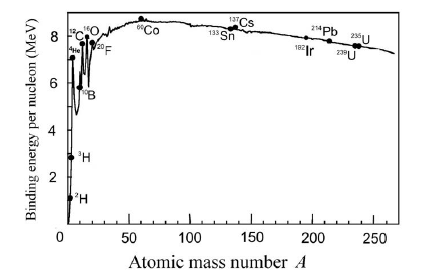
\includegraphics[width=12cm]{image}
    \caption{\textit{Binding energy per nucleon in megaelectronvolts per nucleon against atomic mass number A. Data are from the National Institute of Science and Technology (NIST).}}
\end{figure}

The peculiar shape of the $E_B$/A versus A curve (Figure 1) suggests two
methods for converting mass into energy: (i) fusion of nuclei at low A and
(ii) fission of nuclei at large A:
\begin{itemize}
    \item Fusion of two nuclei of very small mass, e.g. $^2_1H + ^3_1H -> ^4_2He +n$, will
create a more massive nucleus and release a certain amount of energy. Experiments using controlled nuclear fusion for production of energy have so far not been successful in generating a net energy gain, i.e. the amount
of energy consumed is still larger than the amount created. However, fusion
remains an active field of research and it is reasonable to expect that in the
future controlled fusion will play an important role in the production of
electrical power.
\item Fission attained by bombardment of certain elements of large mass (such as
$^{235}U$) by thermal neutrons in a nuclear reactor will create two lower mass
and more stable nuclei, and transform some mass into kinetic energy of the
two product nuclei. Hahn, Strassman, Meitner and Frisch described fission
in 1939, and, in 1942, Fermi and colleagues at the University of Chicago
carried out the first controlled chain reaction based on nuclear fission. Since then, fission reactors have become an important means of production
of electrical power.
\end{itemize}
\subsection*{Radioactivity}
Radioactivity, also known as radioactive decay, nuclear decay, nuclear
disintegration and nuclear transformation, is a spontaneous process by which
an unstable parent nucleus emits a particle or electromagnetic radiation and
transforms into a more stable daughter nucleus that may or may not be stable.
The unstable daughter nucleus will decay further in a decay series until a stable
nuclear configuration is reached. Radioactive decay is usually accompanied by
emission of energetic particles or $\gamma$ ray photons or both.

All radioactive decay processes are governed by the same general
formalism that is based on the definition of the activity \textit{A(t)} and on a characteristic
parameter for each radioactive decay process, the radioactive decay constant $\lambda$ with dimensions of reciprocal time, usually in $1/s$. The main characteristics of
radioactive decay are as follows:
\begin{itemize}
    \item The radioactive decay constant $\lambda$ multiplied by a time interval that is much
smaller than 1/$\lambda$ represents the probability that any particular atom of a
radioactive substance containing a large number \textit{N(t)} of identical radioactive
atoms will decay (disintegrate) in that time interval. An assumption is made
that $\lambda$ is independent of the physical environment of a given atom.
    \item The activity \textit{A(t)} of a radioactive substance containing a large number
\textit{N(t)} of identical radioactive atoms represents the total number of decays
(disintegrations) per unit time and is defined as a product between \textit{A(t)} and $\lambda$,
\end{itemize}

Nuclear transformations are usually accompanied by emission of energetic
particles (charged particles, neutral particles, photons, etc.). The particles released
in the various decay modes are as follows:
\begin{itemize}
    \item Alpha particles in $\alpha$ decay;
    \item Electrons in $\beta$– decay;
\item Positrons in $\beta$+ decay;
\item Neutrinos in $\beta$+ decay;
\item Antineutrinos in $\beta$– decay;
\item Gamma rays in $\gamma$ decay;
\item Atomic orbital electrons in internal conversion;
\item Neutrons in spontaneous fission and in neutron emission decay;
\item Heavier nuclei in spontaneous fission;
\item Protons in proton emission decay.
\end{itemize}

In each nuclear transformation, a number of physical quantities must
be conserved. The most important of these quantities are: (i) total energy,
(ii) momentum, (iii) charge, (iv) atomic number and (v) atomic mass number
(number of nucleons).




\section*{Basics of Radiopharmeceuticals}
Radioactive tracers are made up of carrier molecules that are bonded tightly to a radioactive atom. These carrier molecules vary greatly depending on the purpose of the scan. Some tracers employ molecules that interact with a specific protein or sugar in the body and can even employ the patient’s own cells. For example, in cases where doctors need to know the exact source of intestinal bleeding, they may radiolabel to a sample of red blood cells taken from the patient. They then re-inject the blood and use a SPECT scan to follow the path of the blood in the patient. Any accumulation of radioactivity in the intestines informs doctors of where the problem lies.

For most diagnostic studies in nuclear medicine, the radioactive tracer is administered to a patient by intravenous injection. However a radioactive tracer may also be administered by inhalation, by oral ingestion, or by direct injection into an organ. The mode of tracer administration will depend on the disease process that is to be studied.

Approved tracers are called radiopharmaceuticals since they must meet FDA’s exacting standards for safety and appropriate performance for the approved clinical use. The nuclear medicine physician will select the tracer that will provide the most specific and reliable information for a patient’s particular problem. The tracer that is used determines whether the patient receives a SPECT or PET scan.

Radiopharmaceuticals generally consist of two components, a radioactive element (radionuclide), that permits external scan, linked to a non-radioactive element, a biologically active molecule, drug or cell (red and white blood cells labeled with a radionuclide, for example) that acts as a carrier or ligand, responsible for conducting the radionuclide to a specific organ.

Some characteristics are necessary for considering radiopharmaceuticals clinically useful for imaging: 
\begin{itemize}
    \item The decay of the radionuclide should be in specific ranges of energy emissions (511 keV for positron emission tomography – PET and 100-200 keV for gamma cameras) and in sufficient quantity for tomography detection.
    \item It should not contain particulate radiation (beta emissions, for example), because it increases the radiation dose in patients.
    \item The half-life should be for a few hours only.
    \item The radionuclides should not be contaminated by other radionuclides of the same element nor even its stable radionuclides (carrier-free).
    \item They should have specific activity, and the highest specific activity comes from carrier-free radionuclides.
    \item The radiopharmaceutical should not have toxicity and does not manifest physiological effects.
    \item the radiopharmaceutical should be available for instant usage and easy to compound.
    \item The radiopharmaceutical should reach the target organ quickly and accurately, according to its intended application.
    
\end{itemize}

\section*{Basics of Radiobiology}
Radiobiology is the study (both qualitative and quantitative) of the actions of ionizing radiations on living matter. Since radiation has the ability to cause changes in cells which may later cause them to become malignant, or bring about other detrimental functional changes in irradiated tissues and organs, consideration of the associated radiobiology is important in all diagnostic applications of radiation. Additionally, since radiation can lead directly to cell death, consideration of the radiobiological aspects of cell killing is essential in all types of radiation therapy.

\subsection*{Molecular effect of radiation}
Radiation induced damage to biological targets may result from direct or
indirect action of radiation (Figure 2):

\begin{itemize}
    \item Direct action involves ionization or excitation (via Coulomb interactions) of
the atoms in the biological target. This gives rise to a chain of events which
eventually leads to the observable (macroscopic) damage. In normally
oxygenated mammalian cells, the direct effect accounts for about one third
of the damage for low LET radiations such as electrons and photons.
\item Indirect action involves radiation effects on atoms or molecules which
are not constituent parts of the biological target. Since cells exist in a rich
aqueous environment, the majority of indirect actions involve the ionization
or excitation of water molecules. The free radicals subsequently created
may then migrate and damage the adjacent biological targets. Indirect action
is the main cause of radiation damage and, in normoxic cells, accounts for
about two thirds of the damage.
\end{itemize}

\begin{figure}[htp]
    \centering
    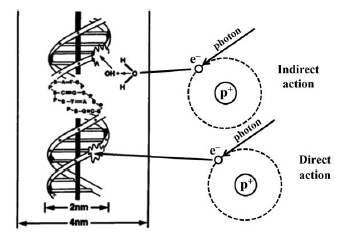
\includegraphics[width=7.8cm]{image_1}
    \caption{\textit{Illustration of the difference between direct and indirect damage to cellular DNA.}}
\end{figure}

\subsection*{DNA Damage}
DNA damage is the primary cause of cell death caused by radiation.
Radiation exposure produces a wide range of lesions in DNA such as single
strand breaks (SSBs), double strand breaks (DSBs), base damage, protein–DNA
cross-links and protein–protein cross-links (see Figure 2). The number of DNA
lesions generated by irradiation is large, but there are a number of mechanisms
for DNA repair. As a result, the percentage of lesions causing cell death is very
small. The numbers of lesions induced in the DNA of a cell by a dose of 1–2 Gy
are approximately: base damages: $>$ 1000; SSBs: $\approx$1000; DSBs: $\approx$40. DSBs play
a critical role in cell killing, carcinogenesis and hereditary effects. There are
experimental data showing that the initially produced DSBs correlate with
radiosensitivity and survival at lower dose, and that unrepaired or misrepaired
DSBs also correlate with survival after higher doses. Furthermore, there is
experimental evidence for a causal link between the generation of DSBs and the
induction of chromosomal translocations with carcinogenic potential.

\subsection*{Concept of cell death}
Radiation doses of the order of several grays may lead to cell loss. Cells
are generally regarded as having been ‘killed’ by radiation if they have lost
reproductive integrity, even if they have physically survived. Loss of reproductive
integrity can occur by apoptosis, necrosis, mitotic catastrophe or by induced
senescence. Although all but the last of these mechanisms ultimately results in
physical loss of the cell, this may take a significant time to occur.

Apoptosis or programmed cell death can occur naturally or result from
insult to the cell environment. Apoptosis occurs in particular cell types after low
doses of irradiation, e.g. lymphocytes, serous salivary gland cells, and certain
cells in the stem cell zone in testis and intestinal crypts.

Necrosis is a form of cell death associated with loss of cellular membrane
activity. Cellular necrosis generally occurs after high radiation doses.

Reproductive cell death is a result of mitotic catastrophe (cells attempt
to divide without proper repair of DNA damage) which can occur in the first
few cell divisions after irradiation, and it occurs with increasing frequency after
increasing doses.

Ionizing radiation may also lead to senescence. Senescent cells are
metabolically active but have lost the ability to divide.

\subsection*{Radiation effects on tumors}
Cells which are lethally affected by radiation may continue to function
for some time after the infliction of the damage, only dying when attempting
to undergo subsequent cell division (mitosis). Clinically observed radiation
effects in whole tissues or organs reflect the damage inflicted to large numbers
of constituent cells and, thus, appear on a timescale which is governed largely
by the underlying proliferation rates of those cells. Such observable effects
are classified as being either late or early, depending on the speed at which
they manifest themselves following irradiation. Late effects appear months or
years after irradiation and appear in structures which proliferate very slowly,
e.g. kidney. Early (or acute) effects appear within days, weeks or months of
irradiation and are associated with fast-proliferating epithelial tissues, e.g. bone marrow, mucosa, intestinal tract, etc.
\subsection*{Imaging the radiobiology of tumors}
The development of molecular imaging using positron emission tomography
(PET) has given rise to new radiotracers which have the potential to assess
several features of radiobiological relevance for therapy planning. One tracer
that is becoming more widely available for PET imaging is fluorothymidine.
This radiotracer exhibits the property of becoming selectively entrapped within
cells that are progressing through S-phase (DNA replication) of the cell cycle,
thus providing a signal which should be proportional to cell proliferation,
and minimizing the signal from cells in G0 or in cell cycle arrest. The ability to
selectively identify only replicating cells separate from all tumour cells present
within the computed tomography-determined tumour volume may present an
excellent opportunity for more accurate measures of the initial viable tumour
burden as well as evaluating tumour response. Complementary to measuring
tumour response is the measurement of therapeutic efficacy through radiotracers
that selectively target cell death. Radiotracers are under development with the
ability to selectively bind to receptors expressed on cells undergoing programmed
cell death, e.g. radiolabelled annexin V. Another area of active research is in the
field of hypoxia imaging. Cells within a tumour microenvironmental region of low
partial oxygen pressure, i.e. hypoxia, are known to exhibit a great radio-resistance
to both radiation and chemotherapy relative to those under normoxic conditions.
A number of PET radiotracers are under evaluation for imaging tumour
hypoxia with PET, including fluoromisonidazole ($^{18}$F-FMISO), fluoroazomycin
arabinoside ($^{18}$F-FA ZA) and copper-diacetyl-bis(N4-methylthiosemicarbazone)
($^{64}$Cu-ATSM). The ability to measure the radiobiological attributes of a tumour
prior to therapy may provide invaluable information concerning the relative
resistance/aggressiveness of tumours, leading to improved management of these
patients.


\section*{References}


1.\url{https://www.redalyc.org/journal/429/42959945001/html/}
\newline
2.\url{https://www.sciencedirect.com/book/9781416051985/physics-in-nuclear-medicine
}
\newline
3.\url{https://www.radiologyinfo.org/en/info/gennuclear}
\newline
4.\url{https://en.wikipedia.org/wiki/Nuclear_medicine
}







\end{document}
